%!TeX program = xelatex

% Define document font, paper size and type %
\documentclass[12pt, numbers=noenddot]{scrreprt}

% Include all auxiliary packages
% All required packages to be used within this project

% Margin definitions
\usepackage[a5paper,vmargin=2cm,hmargin=1.5cm]{geometry}

% Packages to be used
\usepackage{fontspec}
\usepackage{eurosym}
\usepackage{amssymb}
\usepackage{mathtools}
\usepackage{amsmath}
\usepackage{upquote}
\usepackage{microtype}
\usepackage{longtable,booktabs}
\usepackage{graphicx}
\usepackage{grffile}
\usepackage{appendix}
\usepackage{float}
\usepackage{pst-all}
\usepackage{geometry}
\usepackage{xcolor}
\usepackage{xpatch}
\usepackage{nccmath}
\usepackage{subcaption}
\usepackage{xcolor}
\usepackage{multirow}
\captionsetup{compatibility=false}
\usepackage[crop=off]{auto-pst-pdf}
\usepackage[normalem]{ulem}

% Custom links color
\definecolor{linkscolor}{rgb}{0.89, 0.26, 0.2}

\usepackage[unicode=true,bookmarks=true,bookmarksopen=false,
  bookmarksopenlevel=1,pdfborder={0 0 0},backref=false,
  colorlinks=true,allcolors=red,pdfstartview=Fit,
  pdfcenterwindow=true,pdfdisplaydoctitle=true,
  pdfpagelayout=OneColumn,linktocpage=true]{hyperref}
\useunder{\uline}{\ul}{}

% Path for all graphic utilities
\graphicspath{
  {fig/}
}



% Bibliography setup
\usepackage[backend=biber, style=ieee, citestyle=authoryear, sorting=ynt]{biblatex}
\bibliography{bib/sample}

% Custom commands: always the last ones to import to properly override default
% Custom paragraph distance
\setlength{\parskip}{1em plus 2pt minus 1pt}
\setlength{\emergencystretch}{3em}

% Beautiful captions for figures
\captionsetup[figure]{
  format=hang,
  name=Fig.,
  singlelinecheck=off,
  labelsep=colon,
  labelfont=bf,
  font=small
}

% Improve hyperlinks when citing references
\DeclareCiteCommand{\citetitle}
{\boolfalse{citetracker}%
  \boolfalse{pagetracker}%
  \usebibmacro{prenote}}
{\ifciteindex
  {\indexfield{indextitle}}
  {}%
  \printtext[bibhyperref]{\printfield[citetitle]{labeltitle}}}
{\multicitedelim}
{\usebibmacro{postnote}}

\DeclareCiteCommand{\cite}
{\usebibmacro{prenote}}
{\usebibmacro{citeindex}%
  \printtext[bibhyperref]{\usebibmacro{cite}}}
{\multicitedelim}
{\usebibmacro{postnote}}

\DeclareCiteCommand*{\cite}
{\usebibmacro{prenote}}
{\usebibmacro{citeindex}%
  \printtext[bibhyperref]{\usebibmacro{citeyear}}}
{\multicitedelim}
{\usebibmacro{postnote}}

\DeclareCiteCommand{\parencite}[\mkbibparens]
{\usebibmacro{prenote}}
{\usebibmacro{citeindex}%
  \printtext[bibhyperref]{\usebibmacro{cite}}}
{\multicitedelim}
{\usebibmacro{postnote}}

\DeclareCiteCommand*{\parencite}[\mkbibparens]
{\usebibmacro{prenote}}
{\usebibmacro{citeindex}%
  \printtext[bibhyperref]{\usebibmacro{citeyear}}}
{\multicitedelim}
{\usebibmacro{postnote}}

\DeclareCiteCommand{\footcite}[\mkbibfootnote]
{\usebibmacro{prenote}}
{\usebibmacro{citeindex}%
  \printtext[bibhyperref]{ \usebibmacro{cite}}}
{\multicitedelim}
{\usebibmacro{postnote}}

\DeclareCiteCommand{\footcitetext}[\mkbibfootnotetext]
{\usebibmacro{prenote}}
{\usebibmacro{citeindex}%
  \printtext[bibhyperref]{\usebibmacro{cite}}}
{\multicitedelim}
{\usebibmacro{postnote}}

\DeclareCiteCommand{\textcite}
{\boolfalse{cbx:parens}}
{\usebibmacro{citeindex}%
  \printtext[bibhyperref]{\usebibmacro{textcite}}}
{\ifbool{cbx:parens}
  {\bibcloseparen\global\boolfalse{cbx:parens}}
  {}%
  \multicitedelim}
{\usebibmacro{textcite:postnote}}

\DeclareCiteCommand{\citeauthor}%
{\boolfalse{citetracker}%
  \boolfalse{pagetracker}%
  \usebibmacro{prenote}}
{\ifciteindex
  {\indexnames{labelname}}
  {}%
  \printtext[bibhyperref]{\printnames{labelname}}}
{\multicitedelim}
{\usebibmacro{postnote}}

% Reduce top and lower space in equations
\xpatchcmd{\NCC@ignorepar}{
  \abovedisplayskip\abovedisplayshortskip}
{
  \abovedisplayskip\abovedisplayshortskip
  \belowdisplayskip\belowdisplayshortskip}
{}{}

% Do not restart footnotes counter
\counterwithout{footnote}{chapter}

% Custom norm for equations
\DeclarePairedDelimiter{\norm}{\lVert}{\rVert}

% Custom arctan2 and atan2 functions
\DeclareMathOperator{\arctantwo}{arctan2}
\DeclareMathOperator{\atantwo}{atan2}

% Custom piecewise functions
\DeclarePairedDelimiter\Floor\lfloor\rfloor
\DeclarePairedDelimiter\Ceil\lceil\rceil

% Trigonometric functions
\DeclareMathOperator{\sech}{sech}
\DeclareMathOperator{\csch}{csch}
\DeclareMathOperator{\arcsec}{arcsec}
\DeclareMathOperator{\arccot}{arccot}
\DeclareMathOperator{\arccsc}{arccsc}
\DeclareMathOperator{\arccosh}{arccosh}
\DeclareMathOperator{\arcsinh}{arcsinh}
\DeclareMathOperator{\arctanh}{arctanh}
\DeclareMathOperator{\arcsech}{arcsech}
\DeclareMathOperator{\arccsch}{arccsch}
\DeclareMathOperator{\arccoth}{arccoth}

% Custom command for blank page
\newcommand{\blankpage}{\newpage \ \thispagestyle{empty} \newpage}

% Custom command for the table of contents
\newcommand{\maketableofcontents}{\tableofcontents \blankpage \listoffigures \blankpage \listoftables \blankpage}

% Custom command for ESCRIBA
\newcommand{\ESCRIBA}{\href{https://github.com/jorgepiloto/escriba}{ESCRIBA} }


% Start the document
\begin{document}

% Switch off page numbering %
\pagenumbering{Roman}

% Append cover and prologue to actual document %
% Start generating the title page
\begin{titlepage}

  % All content will be centered within this page
  \begin{center}

    % Title of the essay
    \noindent\rule{\textwidth}{1pt}
    \\[0.25cm]
    {
    % Apply font size and color
    \fontsize{35pt}{35pt}\selectfont
    {
      USER GUIDE
    }
    }
    \noindent\rule{\textwidth}{1pt}

    % Add cover logo
    \vspace{2cm}
    \begin{figure}[h]
      \centering
      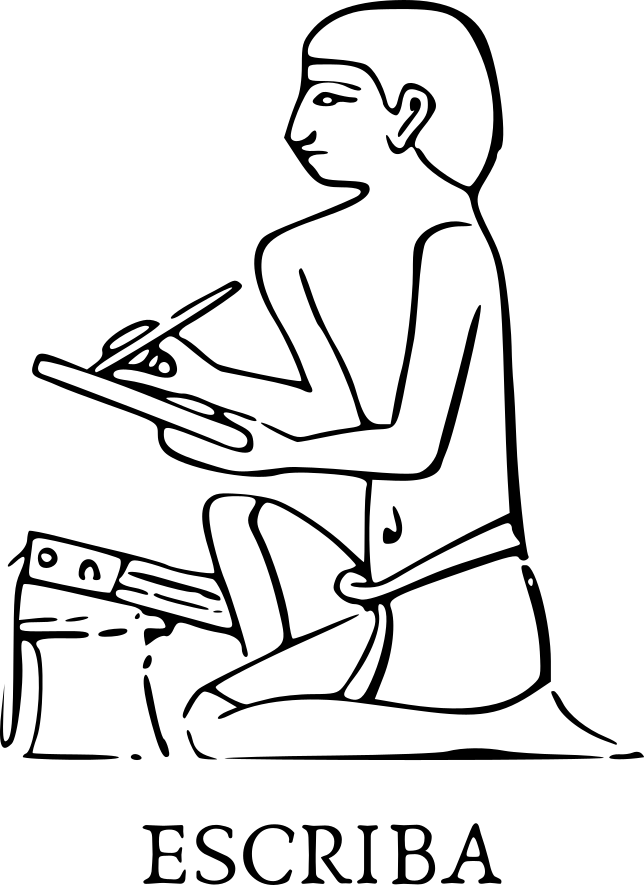
\includegraphics[scale=0.35]{static/logo.png}
    \end{figure}
    \vspace{1.5cm}

    % About
    \textsc{\large
      \textbf{An efficient and automated\\ \LaTeX \ project layout}
    }\\[0.25cm]

  \end{center}
\end{titlepage}

\blankpage
\chapter*{Abstract}

This is the official \ESCRIBA user guide. The tool allows for efficiently manage
large \LaTeX based projects and automate several tasks such us cleaning of the
working directory, code reformatting, linking of externally generated figures
and bibliography compilation.

In this manual, all required information for downloading, installing, creating a
new project and customizing it is presented.

The tool is still under heavy maintenance, so if you experience any issue or bug
while working with it, please open a new issue in the official board:
\href{https://github.com/jorgepiloto/escriba/issues}{https://github.com/jorgepiloto/escriba/issues}.

\vspace{4cm}
\textbf{Keywords:} \LaTeX, automated template, project documentation, academical
work

\blankpage

% Start the table of contents, figures and tables %
\tableofcontents

% ---------- BEGIN OF CONTENT FILES -------------
\pagenumbering{arabic}
\chapter{The ESCRIBA project}

\ESCRIBA is just an efficient and automated \LaTeX project layout:

\begin{itemize}
  \item A project layout because it provides you with several directories
        for building documents making use of \LaTeX.
  \item It is automated, as it ships with a Makefile for cleaning, formatting,
        compiling and rendering your work.
  \item And finally, it is efficient because it saves you time!
\end{itemize}

When working with large academical works, it might be difficult to manage large
quantities of data and information. The only thing writer should care about is
writing. This is the main goal of \ESCRIBA.

In addition, this tool does not require from Ethernet access, meaning that you
can fully work locally and keep track of the changes by using a version control
system (VCS) such is \href{https://git-scm.com/}{Git}.

Finally, \ESCRIBA is an open-source software, released under
\href{https://github.com/jorgepiloto/escriba/blob/main/LICENSE}{Apache 2.0
  LICENSE}. This means that users are allowed to improve and contribute to the
project or even create a new one! The source code is hosted in
\href{https://github.com/jorgepiloto/escriba}{https://github.com/jorgepiloto/escriba}.

\chapter{Installation guide}

This chapter is devoted to explain the user how to install the \ESCRIBA tool.
First all software dependencies are introduced and their own installation guide
is provided. Then, the chapter focuses on how to download and install \ESCRIBA.

\section{Project dependencies}

Before even downloading \ESCRIBA, you require from some additional tools. These
tools or dependencies are for code formatting of drawings compilation and
rendering. Some of those are optional, but it is recommended that you install
all of them.

The required dependencies by \ESCRIBA are:

\begin{itemize}
  \item \href{https://www.gnu.org/software/make/}{Make}: a tool for automating
        processes, originally designed for controlling the generation of
        executables and other non-source files. By making use of a Makefile,
        different rules are provided for managing all your \LaTeX project.
  \item \href{https://www.latex-project.org/}{\LaTeX}: of course, without it you
        will not be able to render any document.
  \item \href{https://www.ghostscript.com/}{Ghostscript (optional)}: used for building
        drawings created by the Asymptote software.
  \item \href{https://asymptote.sourceforge.io/}{Asymptote (optional)}: a framework which
        allows the creation of vectorial drawings by making use of custom
        scripts. It is a very powerful tool for drawing beautiful scientific
        figures which would be complex of getting if using
        \href{https://es.overleaf.com/learn/latex/TikZ_package}{TkiZ}.
  \item \href{https://www.python.org/}{Python}: because \ESCRIBA is a
        \href{https://github.com/cookiecutter/cookiecutter}{cookiecutter} template, you will need this programming
        language to create a new project.
\end{itemize}

From now on, it will be assumed that the operative system you are using is a
Linux based one, in particular the \href{https://ubuntu.com/download}{Ubuntu}
flavor. The only thing which differs from this flavor with the rest is the
package manager you use for installing the dependencies.

\subsection{Installing the dependencies}

For installing the different dependencies, use your favorite package manager. As
said before, Ubuntu is the Linux distribution being used as example. Therefore,
follow the command exposed by figure \ref{fig:install_deps}:

\begin{figure}[h]
  \centering
  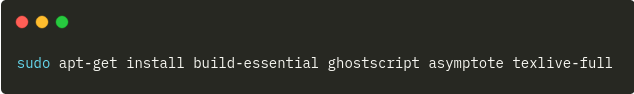
\includegraphics[width=\linewidth]{static/install_deps.png}
  \caption{The command to be used for installing the dependencies.}
  \label{fig:install_deps}
\end{figure}

Regarding Python installation, it is likely that your system already ships with
it. Nevertheless, you can download it from the official Python webpage. To do
so, use the link provided below these lines:

\begin{center}
  Download Python: \href{https://www.python.org/downloads/}{https://www.python.org/downloads/}
\end{center}

Once you have downloaded Python and installed it, it is time for installing the
\href{https://github.com/cookiecutter/cookiecutter}{cookiecutter} package. This
package allows for building templates, so you can start a new \ESCRIBA project
whenever you want. Run the same command from figure
\ref{fig:install_cookiecutter}:

\begin{figure}[h]
  \centering
  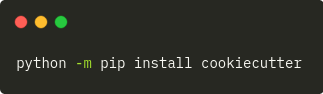
\includegraphics[scale=0.5]{static/install_cookiecutter.png}
  \caption{The command to install cookiecutter package.}
  \label{fig:install_cookiecutter}
\end{figure}


\chapter{How to use ESCRIBA}

This chapter presents to the user how to use \ESCRIBA. At first, the procedure
for creating a new project is presented together with the different available
rules and commands.

\section{Creating a new ESCRIBA project}

After installing all project dependencies, you are ready to download and use
\ESCRIBA. Because this tool is simply a \LaTeX template it does not require from
an installation but from a cookiecutter call. Hence, start a new \ESCRIBA
project by running the command from figure \ref{fig:installing_escriba}:


\begin{figure}[h]
  \centering
  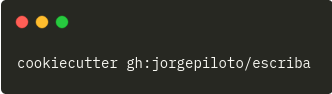
\includegraphics[scale=0.5]{static/install_escriba.png}
  \caption{The command to create a new ESCRIBA project.}
  \label{fig:installing_escriba}
\end{figure}

Previous command will ask you to input some parameters such us the name of your
project, the title of your work, author, location and date among others. These
parameters might become more complex as the project evolves.

\section{Project structure}

Any \ESCRIBA project will generate the structure depicted by figure
\ref{fig:project_layout}.

\begin{figure}[h]
  \centering
  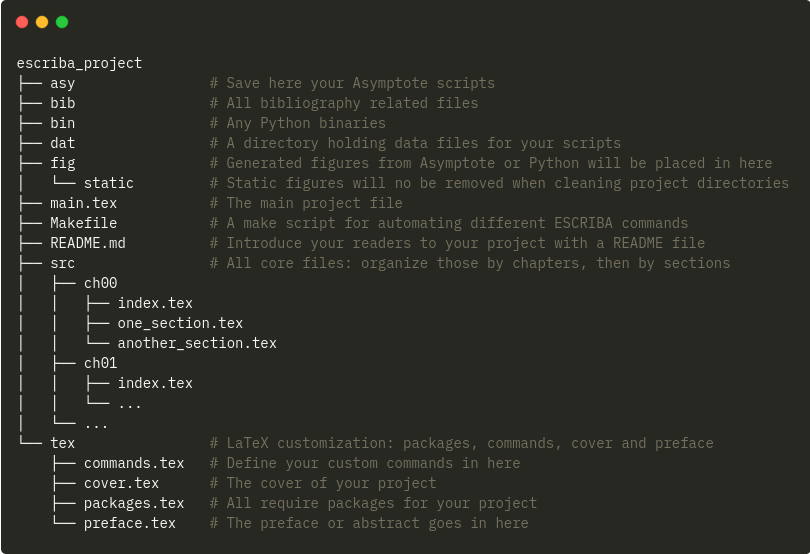
\includegraphics[width=\linewidth]{static/project_layout.png}
  \caption{Generic ESCRIBA project layout.}
  \label{fig:project_layout}
\end{figure}

Each one of the directories is devoted to a particular task:

\begin{itemize}

  \item The main goal of the asy/ directory is to store all the
        \href{https://asymptote.sourceforge.io/}{Asymptote} scripts for generating the different
        vector figures of your project. \ESCRIBA will automatically detect if
        any figure is present, compile it and move it temporary to the fig/
        folder before compiling your \LaTeX document.

  \item The bib/ directory is expected to store all the bibliography files,
        who's extension is *.bib. You will need to link manually those in the
        main.tex file.

  \item Regarding the bin/ folder, it is devoted to the storage of binaries.
        These can be Python files or any other ones. However, for the moment,
        \ESCRIBA is only expected to work with Python scrips.

  \item The dat/ directory can be used to save different data files used by the
        binaries.

  \item For the fig/ folder, every PNG file which is not stored in the
        fig/static/ directory will be assumed to be a temporary file. This is
        because the output of the
        \href{https://asymptote.sourceforge.io/}{Asymptote} scripts or the
        figures developed using the Python binaries are expected to be saved
        in this directory.

  \item The main.tex is the critical file of the project. It links all the
        different *.tex and *.bib files, while declares the \LaTeX class of
        the document. User is expected to add the different index.tex files of
        every chapter within the main.tex.

  \item All the commands and rules are defined in the Makefile. Not only that,
        you can set up the tools and their configuration, such us the
        formatting options or the output name of the rendered PDF.

  \item The README.md is not included but user is encouraged to add one. This is a
        common file in software projects and its goal is to inform users about
        whatever the author considers important about the project.

  \item The src/ directory stores all the information files of the work. The idea
        is that you create a folder for each one of the chapters. Each one of
        these folders is expected to have an index.tex file and one TeX per
        section of the chapter. These content files can be linked using the
        input \LaTeX command in the index.tex. Remember to include the index.tex
        files in the main.tex one. Make sure to include the new chapter
	directories within the \$(CHDIRS) variable in the Makefile.

  \item Finally, the tex/ folder stores some \LaTeX files which are not related to
        the content of your work but to its style, such us the cover, preface or
        abstract and custom commands and packages.

\end{itemize}

\section{Available commands}

As introduced in previous section, the Makefile contains all the rules and
automation commands. Among these rules you can find:

\begin{itemize}
  \item \textbf{make clean}: this rule removes all the auxiliary files generated
	  by \LaTeX, so your project directory becomes clean.
  \item \textbf{make drawings}: this command will compile all the scripts stored
	  in the asy/ directory but will not remove those from the fig/ one.
  \item \textbf{make binaries}: this command will compile all the binaries
	  hosted in the bin/ folder.
  \item \textbf{make reformat}: by calling this rule, all your TeX files will be
	  reformatted according to the options defined in the
	  \$(LATEXINDENTOPTS) variable, which you can modify as you need.
  \item \textbf{make pdf}: the command use to compile and render the whole
	  project into a final PDF file.
\end{itemize}



\chapter{How to customize}


To be completed...


% ----------- END OF CONTENT FILES -------------


% Cite the bibliography
\printbibliography

\end{document}
